\documentclass[a4paper,12pt]{article}
\usepackage{amsmath}
\usepackage{amssymb}
\usepackage[polish]{babel}
\usepackage{polski}
\usepackage[utf8]{inputenc}
\usepackage{indentfirst}
\usepackage{geometry}
\usepackage{array}
\usepackage[pdftex]{color,graphicx}
\usepackage{subfigure}
\usepackage{afterpage}
\usepackage{setspace}
\usepackage{color}
\usepackage{wrapfig}
\usepackage{listings}
\usepackage{datetime}

\renewcommand{\onehalfspacing}{\setstretch{1.6}}

\geometry{tmargin=2.5cm,bmargin=2.5cm,lmargin=2.5cm,rmargin=2.5cm}
\setlength{\parindent}{1cm}
\setlength{\parskip}{0mm}

\newenvironment{lista}{
\begin{itemize}
  \setlength{\itemsep}{1pt}
  \setlength{\parskip}{0pt}
  \setlength{\parsep}{0pt}
}{\end{itemize}}

\newcommand{\linia}{\rule{\linewidth}{0.4mm}}

\definecolor{lbcolor}{rgb}{0.95,0.95,0.95}
\lstset{
    backgroundcolor=\color{lbcolor},
    tabsize=4,
  language=c++,
  captionpos=b,
  tabsize=3,
  frame=lines,
  numbers=left,
  numberstyle=\tiny,
  numbersep=5pt,
  breaklines=true,
  showstringspaces=false,
  basicstyle=\footnotesize,
  identifierstyle=\color{magenta},
  keywordstyle=\color[rgb]{0,0,1},
  commentstyle=\color{green},
  stringstyle=\color{red}
  }

\begin{document}

\noindent
\begin{tabular}{|c|p{11cm}|c|} \hline 
grupa 6 & dariusz szczupak, kamil wanat & \ddmmyyyydate\today \tabularnewline
\hline 
\end{tabular}


\section*{zadanie 4 - liczby pierwsze mpi}

zadanie laboratoryjne polegało na zaimplementowaniu programu sprawdzającego czy podane liczby są liczbami pierwszymi, czy złożonymi. program zaimplementowany zostaz wykorzystaniem języka programowania CUDA C umozliwiającego programowanie z wykorzystaniem procesorow graficznych GPU. Problem został rozwiązany przy pomocy algorytmu ''naiwnego". Jest to metoda nieco wolniesza niż metody probabilistyczne, jednak dająca zdecydowanie lepsze wyniki. Polega ona na dzieleniu testowanego elementu przez kolejne liczby od 2 do pierwiastka kwadratowego z tejże. w naszym programie podejście naiwne zostało nieco zmodyfikowane. zamiast sprawdzać dzielniki od 2 do pierwiastka z każdej liczby, znajdujemy najpierw liczbę maksymalną, a następnie testujemy wszystkie liczby przy pomocy dzielnikow od 2 do sqrt(max). ponadto nie testujemy każdej liczby osobno dla danego dzielnika, lecz cały zbiór. 

\begin{lstlisting}
__global__ void primeTesting (number* tab, uint sqr, uint d)         
{    
uint tid=blockIdx.x;                                                                          
uint i,j;                                                                                     
for (i=2;i<=sqr;i++) {			
        for (j = tid; j <d; j+=gridDim.x) {	
                if((tab[j].value%i==0)&&(tab[j].value!=i)) 
                    tab[j].prime=false;    
        }
    }                                      
}
\end{lstlisting}


Powyzszy kod przedstawia funkcję primeTesting uruchamianą na procesorze graficznym GPU. Odpowiedzialna jest ona za testowanie pierwszosci liczb. Jako argument przyjmuje wskaźnik do obszaru pamięci w ktorym znajdują się dane liczb do testowania, pierwiastek z wartosci maksymalnej liczby, oraz rozmiar danych. Kazdy z watkow odpowiada za sprawdzenie czesci liczb domniemanie pierwszych. Liczby do sprawdzenia przez wątek definiowane są  poprzez zmienną tid - początkowo przyjmującą numer bloku, oraz zwiększaną o calkowitą ilosć blokow. Na kolejnym listingu widoczny jest fragment kopiowania danych do pamięci karty graficznej, wywolanie funkcji jądra oraz kopiowanie powrotne danych do pamięci hosta.

\begin{lstlisting}
    number* tab2;               
    number* temp = tab.data();         
    cudaMalloc( (void**)&tab2, d * sizeof(number) );                     
    cudaMemcpy(tab2, temp, d * sizeof(number), cudaMemcpyHostToDevice);  
    primeTesting <<< blockNumber, 1 >>> (tab2, sqr,d);                    
    number * result;                                                            
    result= (number *) malloc (d*sizeof(number));                               
    cudaMemcpy(result, tab2, d * sizeof(number), cudaMemcpyDeviceToHost);       
\end{lstlisting}

Ponizsza tabela przedstawia zaleznoć przyspieszenia od ilosci blokow wykorzystywanych przez program.
\begin{table}[!hbp]
\centering
\begin{tabular}{|p{5cm}|c|}
\hline 
Liczba blokow & Przyspieszenie \tabularnewline
\hline 
1	& 1\tabularnewline
2	& 1,922430365\tabularnewline
4	& 3,823976317\tabularnewline
8	& 7,628674784\tabularnewline
16 &	15,25149128\tabularnewline
32 &	30,08939713\tabularnewline
64 &	58,210549\tabularnewline
128 &	112,8851456\tabularnewline
256 &	126,3510546\tabularnewline
512 &	151,0486673\tabularnewline
1024 &	152,9736427\tabularnewline
2048 &	164,897505\tabularnewline
4096 &	164,51219\tabularnewline
8192 &	164,7069294\tabularnewline
16384	& 160,7519724\tabularnewline
\hline
\end{tabular}
\caption{Zaleznosć przyspieszenia od ilosci blokow}
\end{table}



\begin{figure}[!hbp]
	\centering
  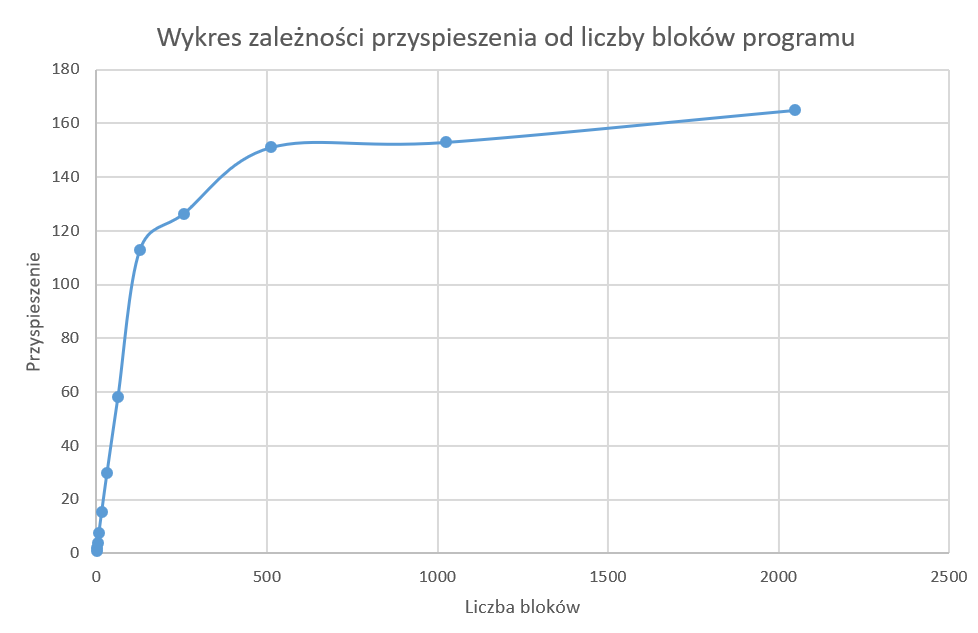
\includegraphics[width=0.7\textwidth]{wykres.png}
  \caption{wykres przyspieszenia}
\end{figure}
wykres przyspieszenia programu testującego liczby pierwsze pokazuje czy i jak udało się zrównoleglić działanie programu. Pierwszą roznicą widoczna w porownaniu do poprzednich zadań jest rozmiar blokow wykorzystanych do zrownoleglenia programu. W poprzednich zadaniach maksymalna liczba procesorow wynosila 12, w tym przypadku liczba ta wzrasta do 16000. Przyspieszenie uzyskane wynosi ponad 150 co w porownaniu do poprzednich technologii jest porazajaca wartoscia. Wykres
 
dane przeprowadzanych testów:
\begin{lista}
 \item wzięto pod uwagę średnią pomiarów czasów wykonania programu dla liczby wątków z przedziału od 1 do 16384. 
 program był uruchamiany dla pliku pobranego z internetu.
 \item do mierzenia czasu wykorzystano zdarzenia CUDA.
 \item testy zostały wykonane na serwerze cuda.iti.pk.edu.pl . 
 \item w czasie testów na serwerze zalogowany był jedynie użytkownik testujący.
\end{lista}


\end{document}

